\documentclass[../report.tex]{subfiles}

\begin{document}

\section{DISTRIBUTED COMPUTING}

\cite{kshemkalyani2011distributed} define \textit{distributed computing} as "characterized as a collection of mostly autonomous processors communicating over a communication network". They identify common features of distributed systems, notably a lack of shared resources which necessitates communication, autonomy and heterogeneity. \\

\begin{figure}[h!]
\centering
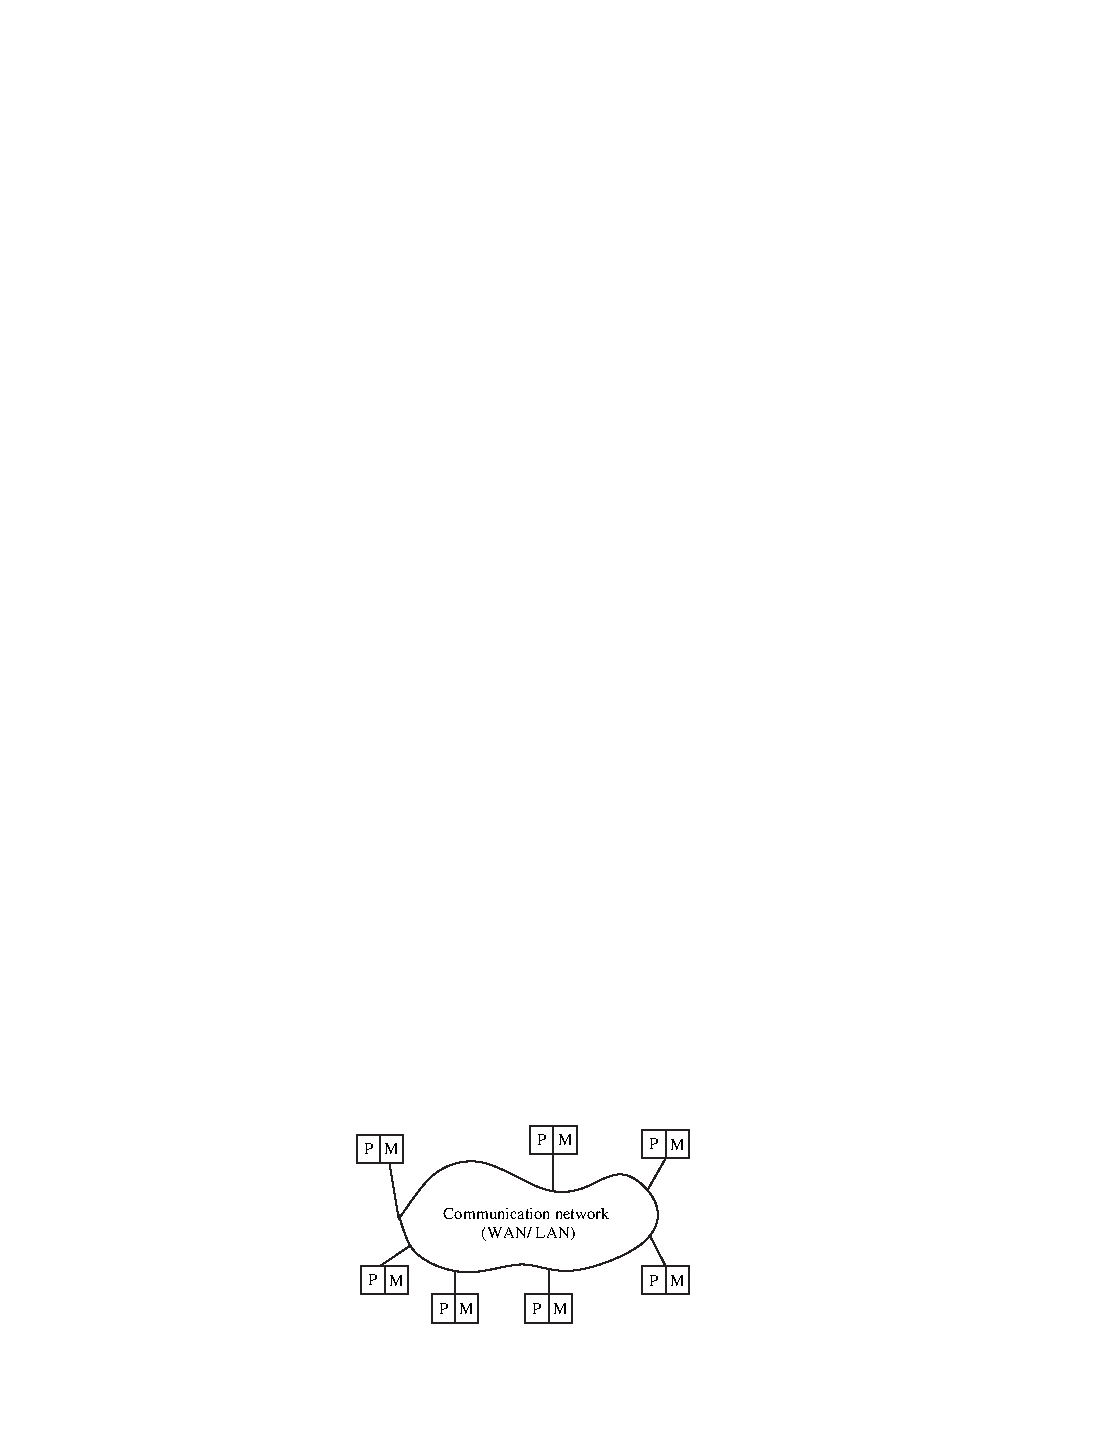
\includegraphics[width=0.8\linewidth]{figures/networkcomms.pdf}
\caption{A distributed system connects processors by a communication network. P = processor(s). M = memory bank(s). \cite[2]{kshemkalyani2011distributed}}
\label{fig:networkcomms}
\end{figure}

\begin{figure}[h!]
\centering
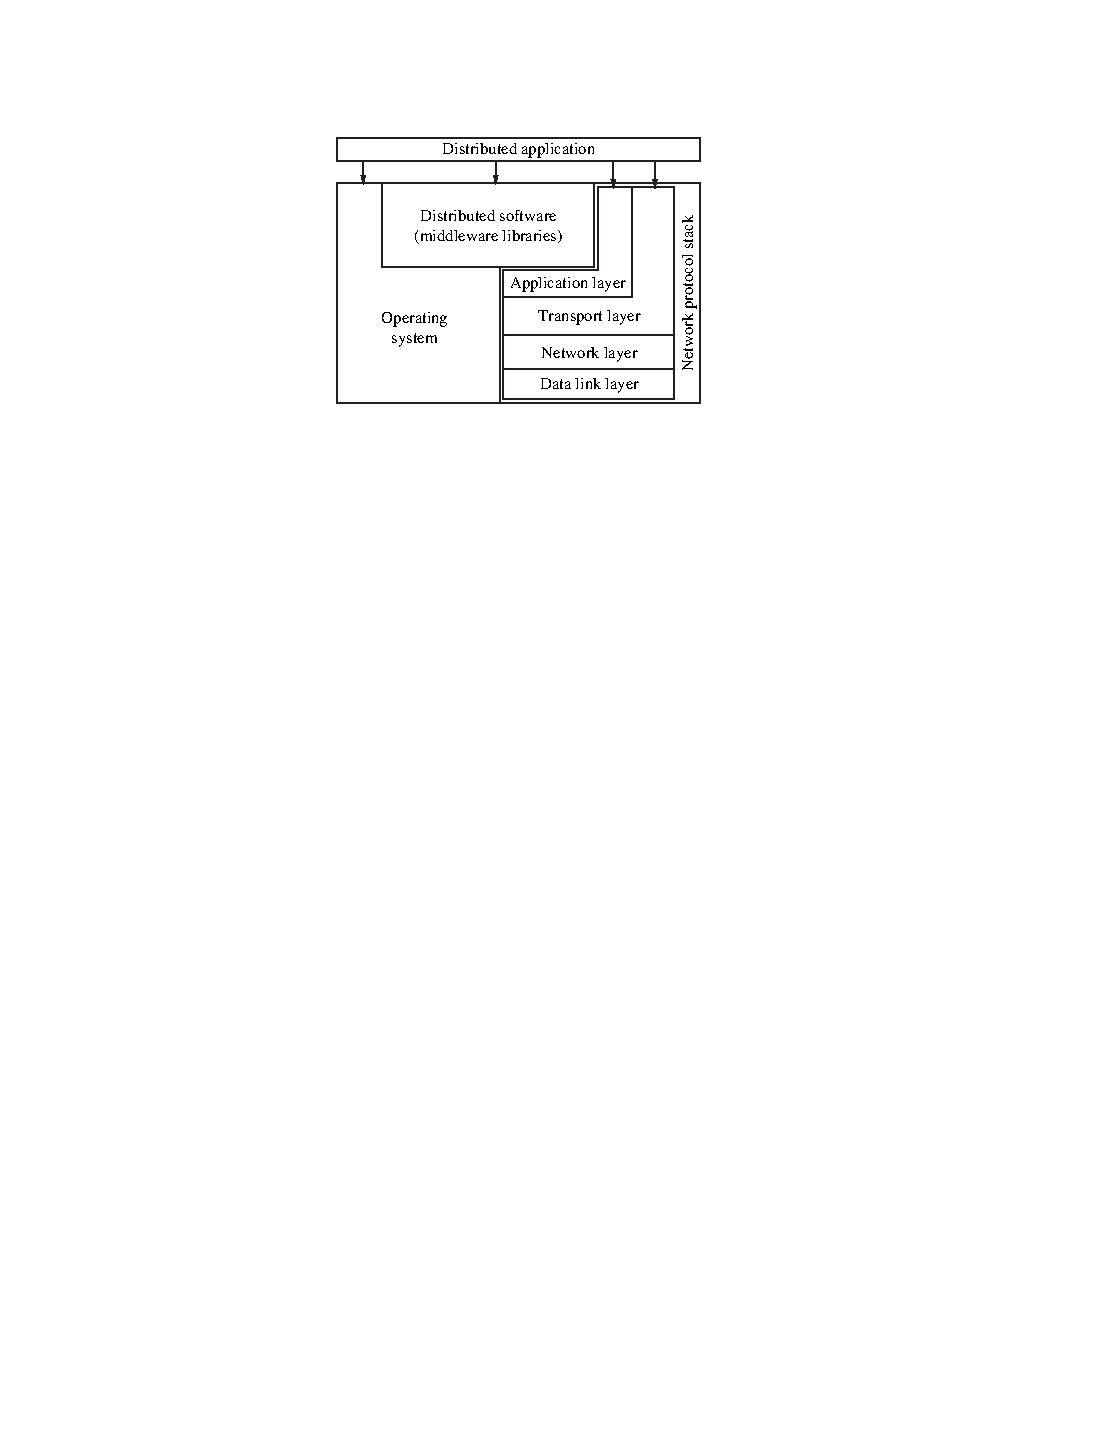
\includegraphics[width=0.8\linewidth]{figures/processinteraction.pdf}
\caption{Interaction of the software components at each processor. \cite[3]{kshemkalyani2011distributed}}
\label{fig:processinteraction}
\end{figure}

\textbf{Distributed computing} (or distributed processing) is the technique of linking together multiple computer servers over a network into a cluster, to share data and to coordinate processing power. Such a cluster is referred to as a “distributed system.” Distributed computing offers advantages in scalability (through a “scale-out architecture”), performance (via parallelism), resilience (via redundancy), and cost-effectiveness (through the use of low-cost, commodity hardware).

As data volumes have exploded and application performance demands have increased, distributed computing has become extremely common in database and application design. This is why it is especially valuable for scaling so that as data volumes grow, that extra load can be handled by simply adding more hardware to the system. Contrast this to traditional “big iron” environments consisting of powerful computer servers, in which load growth must be handled by upgrading and replacing the hardware.

\subsection{Distributed Computing in Cloud Computing}

The growth of cloud computing options and vendors has made distributed computing even more accessible. Although cloud computing instances themselves do not automatically enable distributed computing, there are many different types of distributed computing software that run in the cloud to take advantage of the quickly available computing resources.

Previously, organisations relied on database administrators (DBAs) or technology vendors to link computing resources across networks within and across data centers to be able to share resources. Now, the leading cloud vendors make it easier to add servers to a cluster for additional storage capacity or computing performance.

With the ease and speed in which new computing resources can be provisioned, distributed computing enables greater levels of agility when handling growing workloads. This enables “elasticity,” in which a cluster of computers can be expanded or contracted easily depending on the immediate workload requirements.

\subsection{Key Advantages}

Distributed computing makes all computers in the cluster work together as if they were one computer. While there is some complexity in this multi-computer model, there are greater benefits around:

\textbf{Scalability.} Distributed computing clusters are easy to scale through a “scale-out architecture” in which higher loads can be handled by simply adding new hardware (versus replacing existing hardware).

\textbf{Performance.} Through parallelism in which each computer in the cluster simultaneously handles a subset of an overall task, the cluster can achieve high levels of performance through a divide-and-conquer approach.

\textbf{Resilience.} Distributed computing clusters typically copy or “replicate” data across all computer servers to ensure there is no single point of failure. Should a computer fail, copies of the data on that computer are stored elsewhere so that no data is lost.

\textbf{Cost-effectiveness.} Distributed computing typically leverages low-cost, commodity hardware, making initial deployments as well as cluster expansions very economical.

% Data, Technology, Developers, Users

\pagebreak

\subsection{Data Transmission} % REST APIs

The OSI Model (Open Systems Interconnection Model) is a conceptual framework used to describe the functions of a networking system. The OSI model characterises computing functions into a universal set of rules and requirements in order to support interoperability between different products and software. In the OSI reference model, the communications between a computing system are split into seven different abstraction layers: Physical, Data Link, Network, Transport, Session, Presentation, and Application.

Created at a time when network computing was in its infancy, the OSI was published in 1984 by the International Organisation for Standardisation (ISO). Though it does not always map directly to specific systems, the OSI Model is still used today as a means to describe Network Architecture.

\subsection{The 7 Layers of the OSI Model}

\textbf{Physical Layer.} The lowest layer of the OSI Model is concerned with electrically or optically transmitting raw unstructured data bits across the network from the physical layer of the sending device to the physical layer of the receiving device. It can include specifications such as voltages, pin layout, cabling, and radio frequencies. At the physical layer, one might find “physical” resources such as network hubs, cabling, repeaters, network adapters or modems.

\textbf{Data Link Layer.} At the data link layer, directly connected nodes are used to perform node-to-node data transfer where data is packaged into frames. The data link layer also corrects errors that may have occurred at the physical layer. The data link layer encompasses two sub-layers of its own. The first, media access control (MAC), provides flow control and multiplexing for device transmissions over a network. The second, the logical link control (LLC), provides flow and error control over the physical medium as well as identifies line protocols.

\textbf{Network Layer.} The network layer is responsible for receiving frames from the data link layer, and delivering them to their intended destinations among based on the addresses contained inside the frame. The network layer finds the destination by using logical addresses, such as IP (internet protocol). At this layer, routers are a crucial component used to quite literally route information where it needs to go between networks.

\textbf{Transport Layer.} The transport layer manages the delivery and error checking of data packets. It regulates the size, sequencing, and ultimately the transfer of data between systems and hosts. One of the most common examples of the transport layer is TCP or the Transmission Control Protocol.

\textbf{Session Layer.} The session layer controls the conversations between different computers. A session or connection between machines is set up, managed, and termined at layer 5. Session layer services also include authentication and reconnections.

\textbf{Presentation Layer.} The presentation layer formats or translates data for the application layer based on the syntax or semantics that the application accepts. Because of this, it at times also called the syntax layer. This layer can also handle the encryption and decryption required by the application layer.

\textbf{Application Layer.} At this layer, both the end user and the application layer interact directly with the software application. This layer sees network services provided to end-user applications such as a web browser or Office 365. The application layer identifies communication partners, resource availability, and synchronises communication.

% Formats, Protocols, Blockchain (Git)?

\pagebreak

\subsection{Object Serialisation} % why, state, formats, advantages and disadvantages

\textbf{Serialisation} is the process of converting a data object—a combination of code and data represented within a region of data storage—into a series of bytes that saves the state of the object in an easily transmittable form. In this serialised form, the data can be delivered to another data store (such as an in-memory computing platform), application, or some other destination. The reverse process—constructing a data structure or object from a series of bytes—is \textbf{deserialisation}. The deserialisation process recreates the object, thus making the data easier to read and modify as a native structure in a programming language.

serialisation enables us to save the state of an object and recreate the object in a new location. serialisation encompasses both the storage of the object and exchange of data. Since objects are composed of several components, saving or delivering all the parts typically requires significant coding effort, so serialisation is a standard way to capture the object into a sharable format. With serialisation, we can transfer objects:

\textbf{Over the wire} for messaging use cases

\textbf{From application to application} via web services such as REST APIs

\textbf{Through firewalls} (as JSON or XML strings)

\textbf{Across domains}

\textbf{To other data stores}

\textbf{To identify changes in data} over time

\textbf{While honoring security} and user-specific details across applications

\subsection{JavaScript Object Notation (JSON)}

...

\end{document}
